\capitulo{1}{Introducción}
Durante muchos años, la comunidad científica ha tratado de elaborar modelos predictivos que ayuden en tareas de \textbf{organización industrial.}

La necesidad de precisar métodos de planificación y producción que sean eficientes en tiempo y coste son cada día más importantes en los \textbf{mercados} competitivos actuales \cite{Geurtsen2023ProductionReview}. Para los fabricantes, resulta especialmente crucial disponer de métodos que garanticen la \textbf{optimización} del equipamiento y los recursos empleados, aunque siempre considerando que, en condiciones reales, pueden sucederse eventos impredecibles que hagan peligrar la viabilidad del modelo \cite{Geurtsen2023ProductionReview}.

Los hospitales producen \textbf{servicios}, y desde hace tiempo han empezado a tomar decisiones estratégicas en los servicios que proveen, debido en gran parte al incremento en la oferta de productos sanitarios y nuevos tratamientos disponibles, así como al entorno competitivo que nos rodea.
Por este motivo, las clínicas, como cualquier otra empresa, buscan medidas para reducir costes e impulsar sus demandas financieras \cite{Maleki2023AMoment}.

Si hablamos de \textbf{sanidad privada}, las dos terceras partes de los ingresos de un hospital dependen de las intervenciones quirúrgicas, las cuales constituyen aproximadamente un 40\% del gasto hospitalario\cite{Pham2008SurgicalProblem}.

Los quirófanos forman parte de un entorno muy complejo, conformado por \textbf{múltiples capas}, y condicionado por un gran número de \textit{interacciones sociales, impredictibilidad y baja tolerancia a fallos.} \cite{Rothstein2018OperatingEfficiency}. 

Por otro lado, las irregularidades en el flujo de trabajo dentro del área quirúrgica resultan en perjuicios sobre la \textbf{salud mental de los profesionales}, a menudo motivados por factores como: \textit{amenaza de demandas, alta presión para realizar tareas difíciles, conflicto de intereses...}\cite{Wheelock2015TheTeamwork}.

Por este motivo, incrementar la productividad en los quirófanos tendría una gran influencia en el rendimiento financiero de los mismos, sin dejar de lado algunas consideraciones éticas (\textit{reducción de listas de espera, priorización, equidad en reparto de recursos...}), incrementando la calidad de los servicios y la satisfacción de los pacientes de forma directamente proporcional a las mejoras conseguidas.

El gasto asociado a los quirófanos es uno de los más elevados de cada hospital, por lo que la optimización del proceso resulta crucial de cara a una gestión eficiente de los recursos.
No obstante, el diseño de una planificación quirúrgica resulta muy difícil, debido a una enorme incertidumbre respecto a la duración de las cirugías \cite{Celik2023APrinciple}.

Dentro de los problemas de optimización, si analizamos la literatura encontramos que la planificación quirúrgica ocupa un área especial dentro de esta disciplina.
En función del criterio a mejorar, los investigadores han propuesto diferentes soluciones una vez identificados y analizados los problemas \cite{Gur2018ApplicationOverview}.

Podemos contribuir a la investigación desde diversos puntos de vista, adoptando múltiples estrategias.
Por ello, derivado de disciplinas como la minería o el análisis de datos, se presentan estrategias novedosas que permitan contar con iniciativas prometedoras de cara a lograr la \textbf{eficiencia }\cite{Schouten2023OperatingReview}.
\newpage

\section{Machine Learning y Predicción del Tiempo Quirúrgico}
Planificar quirófanos consiste en asignar bloques de tiempo a cada uno de los pacientes que forman parte de la cartera de servicios de un hospital, de manera que se lleven a cabo las intervenciones maximizando el uso de recursos y minimizando las pérdidas.

Para ello, se han empleado múltiples herramientas cuantitativas que sirven como apoyo la toma de decisiones de los gestores a lo largo de la literatura, aunque a día de hoy prevalece la \textbf{estimación basada en la experiencia} \cite{Brailsford2011ORPerspective} frente a la exploración de nuevas iniciativas basadas en el aprendizaje máquina. 

Si tratamos de \textit{minimizar el error humano} a la hora de estimar la duración de una intervención quirúrgica determinada, existen varios estudios que aplican diversos algoritmos \textbf{predictivos} a este problema, y comparan su rendimiento entre ellos y respecto al cálculo aplicando exclusivamente la experiencia del gestor.

Por ejemplo, en un estudio reciente \cite{Master2017ImprovingLearning} basado en la población pediátrica, llegaron a la conclusión de que los algoritmos basados en \textbf{árboles} para la predicción basada en variables categóricas (Sexc, raza, edad, diagnóstico, riesgo anestésico...) obtienen menor error predictivo que el uso de las técnicas convencionales de predicción basadas en la experiencia.

Por otro lado, en otro estudio que exploró hasta nueve especialidades quirúrgicas \cite{Martinez2021MachinePrediction} e incorporó variables como el identificador del cirujano responsable y su experiencia, comparó cuatro modelos de ML (Regresión Lineal, SVM, Árboles de Regresión y Bagged Trees), obteniendo \textbf{mejores métricas} que los estudios previos en todos los modelos, concluyendo que los mejores resultados se obtuvieron con Bagged Trees.

Hasta el momento, podemos afirmar que los algoritmos de ML son capaces de predecir la duración de los quirófanos, aunque no hay ninguna solución definitiva, y el rendimiento de los modelos depende, fundamentalmente, del conjunto de datos que sirva como objeto de entrenamiento, así como al servicio de aplicación y sus características intrínsecas.

\newpage
\section{Optimización en Planificación}
Tal y como hemos reseñado en apartados anteriores, planificar quirófanos consiste en asignar recursos hospitalarios a casos quirúrgicos individuales en función del tiempo estimado para completar la cirugía, por lo que muchos autores han comparado su resolución como una extensión de un problema de Job Shop, proponiendo modelos de programación lineal para su resolución \cite{Pham2008SurgicalProblem} .

No obstante, los autores difieren en cada uno de los estudios, y parecen aplicar las técnicas de optimización que más encajan con la modelización de su problema, existiendo pocas revisiones en la literatura referentes a la planificación y programación de quirófanos \cite{Gur2018ApplicationOverview}. 

\subsection{Características de los Pacientes}
La mayor parte de los estudios existentes en la literatura dividen sus herramientas de planificación en función de la \textbf{electividad} de los pacientes: Electivos (\textit{programados}) y No Electivos (\textit{urgentes, emergentes, hospitalizados...}).

Debido a la incertidumbre del segundo grupo, éstos no forman parte de antemano de las planificaciones de los gestores, aunque su aparición imprevista genera que se les dé una prioridad máxima a su llegada y se desplace la de los otros grupos en el proceso \cite{CAYIRLI2009OUTPATIENTLITERATURE} .

Aunque existen estudios que tienen en cuenta a ambos grupos y desarrollan medidas de planificación, no existen estudios robustos en la literatura que \textbf{combinen} ambos casos, centrándose en uno de ambos, en función de las características de cada hospital \cite{Gur2018ApplicationOverview}.

Sin embargo, los investigadores tienden a centrar sus esfuerzos en desarrollar medidas de optimización considerando principalmente el primer grupo de pacientes, replanificando si es necesario en el caso de que lleguen casos urgentes o emergentes \cite{Nouaouri2011OperatingDisaster}, teniendo en cuenta que la evaluación de cualquiera de los grupos debe reflejar tanto los tiempos de espera de los pacientes, así como el efecto de la sobrecarga de trabajo en los trabajadores y recursos del entorno hospitalario \cite{Gur2018ApplicationOverview}.

En nuestro trabajo, y siguiendo la estela de la mayor parte de los autores, nos hemos centrado en las medidas de optimización de pacientes \textbf{electivos}, dada la complejidad y la dificultad de obtención de datos en las fuentes consultadas que nos permitan asumir la incertidumbre de diseñar un modelo que tenga en consideración a ambos grupos y ofrezca un rendimiento aceptable.

\subsection{Métricas de Rendimiento}
Antes de desarrollar cualquier medida que tenga como objetivo alcanzar una mejora de \textbf{rendimiento en la planificación quirúrgica (\textit{OR performance})}, debemos definir qué entendemos por rendimiento y, en su caso, \textit{cómo medirlo}. 

Algunas de las más importantes son los referidos en \ref{Métricas de Quirófano}.
\begin{table}[]
    \centering
    \begin{tabular}{c|c}
        \toprule
            \textbf{Métrica}   &  \textbf{Descripción}  \\
         \midrule
              \textit{Hora de Comienzo}  &  Retraso o anticipo en el comienzo de la actividad quirúrgica. \\
              \textit{Tiempo de Recambio }& Tiempo entre cada uno de los pacientes. \\
              \textit{Uso del bloque} & Proporción del tiempo asignado que se dedica a la realización de la actividad. \\
              \textit{Tasa de Cancelaciones} & Las suspensiones o cancelaciones suponen tiempo de actividad desaprovechado. \\
       \bottomrule
    \end{tabular}
    \caption{Métricas de Quirófano}
    \label{Métricas de Quirófano}
\end{table}

No obstante, las métricas usadas para cuantificar el rendimiento de las medidas de optimización en quirófano son muy diversas a lo largo de la literatura.
Muchos artículos focalizan la eficiencia en aspectos meramente cualitativos, mientras que otros se centran en mejorar las métricas más objetivas, buscando la minimización del malgasto de recursos y la correcta gestión del tiempo. \cite{Schouten2023OperatingReview}.

Además, debemos tener en consideración que, mientras que estas medidas de rendimiento personalizan la estructura del problema, también limitan su tamaño, pues cuanto mayor es el número de los criterios de evaluación, la estructura será de mayor tamaño y complicación \cite{Gur2018ApplicationOverview}. 

En nuestro caso, optaremos por \textbf{maximizar} la tasa de utilización del sitio quirúrgico y \textbf{minimizar} los tiempos de espera, teniendo en cuenta las restricciones en cuanto a la ponderación de su prioridad, que definiremos formalmente en apartados posteriores de la memoria. 

\tablaSmall{Eficiencia y Calidad}{c|c}{EficienciayCalidad}
{ \textbf{Eficiencia}  &  \textbf{Calidad} \\}{ 
Maximizar utilización y reducción de retrasos y esperas & Calidad en cuidados\\ 
                                            & Seguridad del paciente\\ 
                                            &  Bienhacer profesional.\\ } 

Podemos resumir, por tanto, que un correcto rendimiento debe satisfacer requisitos de \textbf{eficiencia }y \textbf{calidad} \cite{Sandbaek2014ImpactEfficiency}.


\subsection{Alcance de la Planificación}
Si tenemos en consideración la bibliografía disponible hasta el momento, encontramos cómo la tarea de planificación llega a incluir, en algunos estudios, el uso de áreas como la Unidad de Reanimación Postanestésica o la de Cuidados Intensivos, como parte del proceso, pudiendo mejorar el rendimiento desde el punto de vista estratégico a largo plazo \cite{Gur2018ApplicationOverview}.

No obstante, la mayor parte de los autores no tienen en cuenta estas características y la mayor parte de los avances realizados en la materia se centran en el uso exclusivo del área quirúrgica, dejando para investigaciones futuras la inclusión del resto de facilidades hospitalarias en el cómputo final.

Por otro lado, los recursos del quirófano suelen ser reconocidos como una unidad, aunque algunos estudios como \cite{DiMartinelly2014AnScheduling} tuvieron en consideración la \textbf{dotación de personal de enfermería }como parte de los recursos a optimizar en el quirófano, no llegando a obtener conclusiones relevantes sobre su importancia en el modelo, siendo las diferencias de rendimiento no significativas respecto a su inclusión tradicional en el bloque.

Es por estos motivos por los que hemos decidido centrar nuestros esfuerzos en la elaboración de un modelo de gestión centrado en la \textbf{sala de operaciones} y considerando los recursos disponibles como un único elemento indivisible, tanto en las tareas de predicción como en las de planificación.

\subsection{Técnicas de Optimización}
Las medidas computacionales empleadas en gran parte de los estudios tienen como objetivo la minimización del tiempo de espera de los pacientes y el coste hospitalario, junto a la maximización del tiempo de utilización de la sala quirúrgica.

Podemos encontrar gran número de aproximaciones, dado que el problema a modelar es NP-Complejo (ILP). Desde metaheurísticas específicas para un entorno concreto, hasta alternativas genéricas como algoritmos genéticos, recocido simulado, colonias de hormigas, particle swarm, programación dinámica... 

En una revisión reciente \cite{Gur2018ApplicationOverview}, la mayor parte de las aproximaciones fueron por \textit{simulación basada en la experiencia} y usando modelos de programación entera mixta (MILP).


\begin{figure}
    \centering
    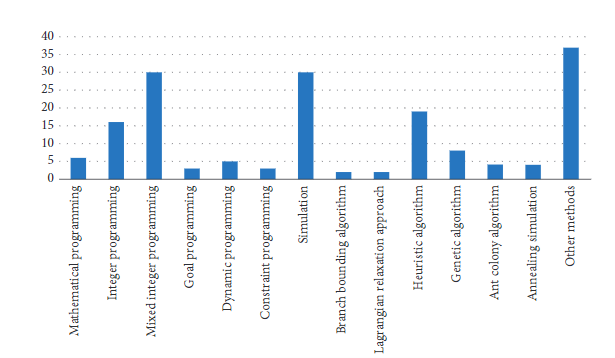
\includegraphics{Memoria TFG/img/graficoAlgoritmos.png}
    \caption{Técnicas de Optimización. Fuente \cite{Gur2018ApplicationOverview}}
    \label{GraficoTecnicasOpt}
\end{figure}

Una vez formulado el problema con nuestras restricciones, probaremos diferentes modelizaciones y algoritmos de planificación durante el transcurso del proyecto, eligiendo finalmente el que nos ofrezca mejor rendimiento de cara a la implementación final de la herramienta.